\documentclass[parskip=half, fontsize=12pt, fleqn]{scrartcl}

% \usepackage[english]{babel}         % Deutsches Sprachpaket

\usepackage{iftex}
\ifPDFTeX
   \usepackage[utf8]{inputenc}% Eingaben codieren
   \usepackage{fourier}
   % \usepackage[T1]{fontenc}   % Umlaute codieren, Silbentrennung
\else
   \usepackage{lmodern}
   % \usepackage[no-math]{fontspec}
   % \setmainfont{Utopia Std}
\fi

\usepackage{amsmath, amssymb}       % Mathe, \mathbb{R}
\usepackage{amsthm,amstext}         % Theoreme, \text im Mathe-Modus
\usepackage{mathtools}              % \Aboxed für Boxen in Align Umgebungen
\usepackage[arrowdel]{physics}      % Ableitungen \dv{B}{t} \pdv \dd{t}
\usepackage[left=2.5cm, right=2.5cm, top=3cm, bottom=3cm]{geometry}
\usepackage{graphicx}               % \includegraphics
\usepackage[extendedchars]{grffile} % extends file name processing of graphics
\usepackage[section]{placeins}      % \Floatbarrier
\usepackage{wrapfig}                % Bilder umfließen
\usepackage{enumerate}              % Aufzählungen
\usepackage{enumitem}               % \begin{enumerate}[label=\alph*]
\usepackage{footnote}               % Fußzeilen
\usepackage{booktabs}               % publication quality tables
\usepackage{tikz, pgfplots}         % TIKZ ist kein Zeichenprogramm
\usepackage[europeanvoltages,europeanresistors]{circuitikz}
\usepackage{bm}                     % bold symbols \bm{r}
\usepackage{dsfont}                 % identity matrix \mathds{1}
\usepackage{esint}                  % Doppelintegrale
\usepackage{mathrsfs}               % \mathscr{} statt \mathcal{}
\usepackage{placeins}               % FloatBarrier
\usepackage{subcaption}
\usepackage{multirow}
\usepackage{mdframed}               % Deckblatt
\usepackage{xcolor}                 % Deckblatt
\usepackage{fancyhdr}               % Kopfzeile
\usepackage{aligned-overset}        % Ausrichtungen mit stackrel oder overset
\usepackage{cancel}
\usepackage{float}
\usepackage{cite}
\usepackage[version=4]{mhchem}                 % Chemistry Package
\usepackage{multicol}
% \usepackage{pdfpages}             % insert whole pdf files

\definecolor{FSUblau}{cmyk}{1,0.7,0.1,0.5}
\definecolor{PAForange}{cmyk}{0.1,0.7,1,0}
\definecolor{Gruen}{cmyk}{1,0.1,0.7,0.5}

\usepackage[final,
    pdfauthor={Martin Beyer},
    pdffitwindow=false,     % resize document window to fit document size
    pdftoolbar=false,        % Adobe Toolbar
    bookmarks=true,         % Anzeigen der Kapitel
    bookmarksopen=true,
    bookmarksopenlevel=0,
    bookmarksnumbered=true,
    colorlinks=true,        % fuer Druckversion auf "false"
    linkcolor=FSUblau,         % Table of Contents, Footnotes
    urlcolor=FSUblau,          % fuer eingebunden URLs
    citecolor=FSUblau,         % Equations, References
    filecolor=FSUblau,
    pdfborder={0 0 0},      % keine Rahmen um Verlinkungen: {0 0 0}
    pagebackref=false
]{hyperref}

\pgfplotsset{compat=1.18}
\newcommand\mydots{\makebox[1em][c]{.\hfil.\hfil.}}
\newcommand{\minus}{\scalebox{0.75}[1.0]{$-$}}
\newcommand{\e}{\mathrm{e}}
\renewcommand{\i}{\mathrm{i}}

\usepackage[detect-all,
            locale=DE,
            exponent-product = \cdot,
            per-mode=fraction]{siunitx}
\usepackage[position=below,
            format=hang,
            figurename=Fig.,
            labelfont={bf},
            font=small]{caption}

\sisetup{range-phrase = {\mydots}}
% Commands
\usetikzlibrary{positioning,intersections,calc,external}
\usepgfplotslibrary{fillbetween, groupplots}
\pgfplotsset{
tick label style={font=\small},
label style={font=\small},
legend style={font=\footnotesize},
every axis post/.style={legend cell align={left}}}
\tikzstyle{every node}=[font=\small]


\setlength{\parindent}{0px}         % keine Absätze durch Leerzeilen im Code
\numberwithin{equation}{section}

% Remove page number from \thispagestyle{empty}
\makeatletter\let\ps@plain\ps@fancy\makeatother

% Deckblatt
\newcommand{\HRule}{\rule{\linewidth}{0.5mm}}
\newcommand{\Deckblatt}[5][\LaTeX-Satz und Design von Martin Beyer]{
  \begin{titlepage}
    \center
    \textsc{\LARGE Friedrich-Schiller-Universität Jena\\[1ex]
    \Large Physikalisch-Astronomische-Fakultät}
    \begin{figure}[h!]
       \centering
       \includegraphics[scale=0.75]{uni-Logo_neu.pdf}
    \end{figure}\\
    \vspace{2em}
    \textsc{\Large #2}\\[0.35cm]
    \HRule \\[0.4cm]
    { \Huge \bfseries #3}\\[0.15cm]
    \HRule \\[0.5cm]
    \textsc{\Large #4}\\[0.35cm]
    \vfill
    \begin{mdframed}[backgroundcolor=gray!20]
      \begin{center}
        #1
      \end{center}
    \end{mdframed}
  \end{titlepage}

  \pagestyle{fancy}
  \fancyhead[R]{\textbf{#5}}
  \fancyfoot[C]{\bfseries\thepage}
  \fancyhead[L]{\rightmark}

  \fancypagestyle{plain}{
    \fancyfoot[C]{\bfseries\thepage}
    \fancyhead[R]{}
    \fancyhead[L]{}
    \renewcommand{\headrulewidth}{0pt}
  }
}
\renewcommand{\sectionmark}[1]{\markright{#1}}
\renewcommand{\headrulewidth}{0.5pt}
\renewcommand{\footrulewidth}{0.5pt}

\newgeometry{left=2cm, right=2cm, top=2cm, bottom=2.5cm}
\setenumerate{labelindent=1em,labelsep=0.5cm,leftmargin=*}

\everymath{\displaystyle}
% no numbering of align environments
\makeatletter
\renewcommand\tagform@[1]{}
\makeatother

\newcommand{\Semester}{2023/24}
\newcommand{\Titelbanner}[2]{
    \begin{center}
        \textsc{
        \LARGE Auffrischungskurs Mathematik\\[0.5cm]
        \large  -- Kurzlösungen zur Selbstkontrolle --\\[0.5cm]}
        \footnotesize WS \Semester
    \end{center}
    \paragraph{Thema #1:} \hspace{0.2cm}
    \begin{minipage}[t]{0.8\linewidth}
        #2
    \end{minipage}
    \vspace{0.7cm}
}

%%%% 
% \includeonly{Lösungen_kurz/Thema_07}
%%%%

\begin{document}
\graphicspath{{./Bilder/}{../}}

\pagestyle{plain}
\renewcommand{\headrulewidth}{0pt}
\pagenumbering{gobble} % no page numbers

\Titelbanner{1}{Grundrechenarten\\
                Brüche\\
                Potenzen\\
                Wurzeln}

\begin{minipage}[t]{0.6\linewidth}
    \textbf{Aufgabe 1: } \emph{Bruchrechnung}
    \begin{enumerate}[label=(\alph*)]
        \item $b-a$
        \item $\dfrac{a}{b}$
        \item $\dfrac{x}{y}-1$
        \item $\dfrac{n^2}{n-1}$
        \item $\dfrac{x+y}{x-y}$
        \item $1$
        \item $\dfrac{a^2}{\sqrt{2}}$
    \end{enumerate}
\end{minipage}
\hfill
\begin{minipage}[t]{0.37\linewidth}
    \textbf{Aufgabe 2: } \emph{Potenzgesetze}
    \begin{enumerate}[label=(\alph*)]
        \item $\left( \dfrac{a+b}{x-y} \right) ^n$
        \item $a^xb^yc^z$
        \item $(a+b)a^2b^{n-2}$
        \item $(a-1)a^{n-2}$
        \item $\dfrac{x^5}{a^{14}b^{19}y^{12}}$
    \end{enumerate}
\end{minipage}\\[2cm]
%
\begin{minipage}[t]{0.6\linewidth}
\textbf{Aufgabe 3: } \emph{Umformungen mit Wurzelausdrücken}
    \begin{enumerate}[label=(\alph*)]
        \item $\dfrac{1+ab}{1-ab}$
        \item $\dfrac{1}{m}$
        \item $a\left(\sqrt[4]{ab}+\sqrt{b}\right)$
    \end{enumerate}
\end{minipage}
\hfill
%
\begin{minipage}[t]{0.4\linewidth}
\textbf{Aufgabe 4: } \emph{Algebraische Umformungen}
    \begin{enumerate}[label=(\alph*)]
        \item $x=\dfrac{1}{(a-b)(m+n)}$
        \item $x=\dfrac{a-b}{a+b}$
        \item $x=\dfrac{3}{4}$
        \item $x=(a+b)^2$
        \item $x=\left|y^2-1\right|$
    \end{enumerate}
\end{minipage}
\Titelbanner{2}{Lineare Gleichungssysteme}

\textbf{Aufgabe 1: } \emph{Zwei lineare Gleichungen mit zwei Unbekannten}
\begin{enumerate}[label=(\alph*)]
    \item $\{(x\,;y)\} = \qty{\qty(\frac{7}{11}\,;\frac{1}{3})}$
    \item $\{(x\,;y)\} = \qty{\qty(\frac{1}{3}\,;\frac{1}{4})}$
    \item $\{(x\,;y)\} = \qty{\qty(-1\,;0)}$
    \item $\{(x\,;y)\} = \qty{\qty(\frac{b}{a}+1\,;\frac{a}{b}-1)}$
    \item $\{(x\,;y)\} = \qty{\qty(\frac{1}{\sqrt{2}}\,;-\frac{1}{\sqrt{2}})}$
    \item $\{(x\,;y)\} = \qty{\qty(a(a+b)\,;b(a-b))}$
    \item $\{(x\,;y)\} = \qty{\qty(\frac{1}{13}\,;\frac{1}{19})}$
\end{enumerate}
\vspace{0.7cm}
%
\textbf{Aufgabe 2: } \emph{Drei Gleichungen mit drei Unbekannten}
\begin{enumerate}[label=(\alph*)]
\item $\{(x\,;y\,;z)\} = \{(1\,;1\,;1)\}$
\item $\{(x\,;y\,;z)\} = \{(1\,;2\,;3)\}$
\item $\{(x\,;y\,;z)\} = \{(a\,;b\,;c)\}$
\item $\{(x\,;y\,;z)\} = \{(2z\,;5z\,;z)\ |\ z\in\mathbb{R}\}$
\end{enumerate}
\vspace{0.7cm}
%
\textbf{Aufgabe 3: } \emph{Parametrisierung von Lösungsmengen}
\begin{enumerate}[label=(\alph*)]
\item $\{(x\,;y)\} = \qty{\qty(\frac{1+7\lambda}{13}\,;\lambda)\ |\ \lambda\in\mathbb{R}}$
\item $\{(x\,;y)\} = \{(6+7n\,;11+13n)\ |\ n\in\mathbb{N}_0\}$
\end{enumerate}
\vspace{0.7cm}

\textbf{Aufgabe 4: } \emph{Gleichungssysteme}
\begin{enumerate}[label=(\alph*)]
\item $\{(x\,;y)\}=\{(2\,;4),(4\,;2)\}$
\item $\{(x\,;y)\}=\{(17\,;6)\}$
\item $\{(x\,;y)\}=\{(-3\,;-3),(-1\,;1)\}$
\end{enumerate}
\vspace{0.7cm}

\textbf{Aufgabe 5: }\emph{Ungleichungssysteme}
\begin{enumerate}[label=(\alph*), labelindent=1em,labelsep=0.5cm]
\item$~$\\[-0.4cm]
\begin{minipage}{0.2\textwidth}
    \begin{alignat*}{3}
        2x-3y&\geq -6\,,\\
        x-2y&< 11\,,\\
        x&>-y-1\,,\\
        x&<5\,,\\
        x&\geq 0\,,\\
        y&\geq 0
    \end{alignat*}
\end{minipage}
\begin{minipage}{0.8\textwidth}
    \centering
        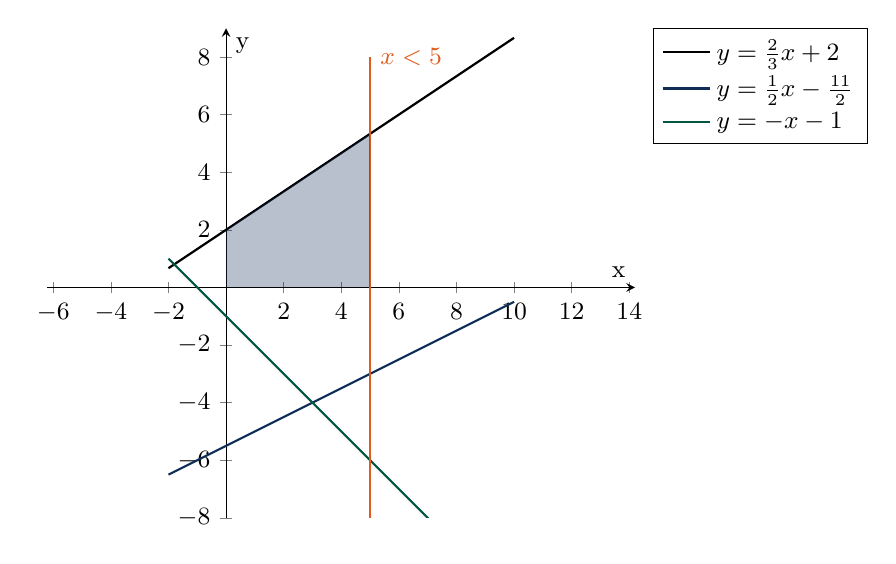
\begin{tikzpicture}
            \begin{axis}[disabledatascaling, axis lines=middle, xlabel={x}, ylabel={y}, height=7.8cm, domain=-2:10, xmin=-3,xmax=11, ymin=-8, ymax=9, axis equal, legend pos= outer north east]
                \addplot[no marks, black, thick, ]{2/3*x+2};
                \addplot[no marks, FSUblau, thick]{0.5*x-11/2};
                \addplot[no marks, Gruen, thick]{-x-1};
                \draw[thick, PAForange, thick] (5,-8)--(5,8)node[right]{$x<5$};
                \fill[FSUblau, fill opacity =0.3] (0,0)--(5,0) --(5,16/3) -- (0,2) -- cycle;
                \legend{$\textstyle y = \frac{2}{3}x+2$, $\textstyle y = \frac{1}{2}x-\frac{11}{2}$, $\textstyle y = -x-1$};
            \end{axis}
        \end{tikzpicture}
\end{minipage}
Offenbar können die zweite und dritte Ungleichung weggelassen werden, ohne dass sich etwas am eingefärbten Gebiet ändert. 

\item Die Ungleichungen beschreiben eine dreiseitige, unendlich ausgedehnte Pyramide, deren Spitze im Koordinatenursprung sitzt und deren Seiten jeweils die $x$-$y$-, $x$-$z$- und $y$-$z$-Ebene halbieren.\\
\begin{center}
\includegraphics[scale=0.25]{entropy_cone.pdf}
\end{center}

\end{enumerate} 
\Titelbanner{3}{Quadratische Gleichungen und Gleichungssysteme}

\begin{minipage}[t]{0.52\textwidth}
    \textbf{Aufgabe 1: } \emph{Quadratische Gleichungen}
    \begin{enumerate}[label=(\alph*)]
        \item $x_1=9\,;\ x_2=1$
        \item $x_1=3\,;\ x_2=-4$
        \item $x_{1/2}=\pm 1+\sqrt{2}$
    \end{enumerate}
\end{minipage}
\hfill
\begin{minipage}[t]{0.48\textwidth}
    \textbf{Aufgabe 3: } \emph{Gleichungssysteme}
    \begin{enumerate}[label=(\alph*)]
    \item $\{x\,;y)\}=\{(4\,;\pm\sqrt{3})\,,(3\,;\pm2)\}$
    \item $\{(x\,;y)\}=\{(1\,;5)\,,(5\,;1)\,,(2\,;3)\,,(3\,;2)\}$
    \item $\{(x\,;y)\}=\{(0\,;0)\,,(-2\,;-4)\,,(4\,;2)\}$
    \end{enumerate}
\end{minipage}
%
\\$~$\\[5mm]
%
\begin{minipage}[t]{0.52\textwidth}
    \textbf{Aufgabe 2: } \emph{Wurzeln quadratischer Gleichungen}
    \begin{enumerate}[label=(\alph*)]
    \item Faktoren $x=\frac{a}{b}-1$ und $y=\frac{b}{a}+1$
    \item $k=\pm3\sqrt{5}$
    \item $\{(p\,;q)\}=\{(0\,;0)\,,(1\,;-2)\}$
    \item 
    \begin{itemize}
    \item $ax^2+2bx+4c=0$
    \item $cx^2+bx+a=0$
    \end{itemize}
    \end{enumerate}
\end{minipage}
\hfill 
\begin{minipage}[t]{0.48\textwidth}
    \textbf{Aufgabe 4: } \emph{Wurzelgleichungen}
    \begin{enumerate}[label=(\alph*)]
    \item $x_1=1\,,\ x_2=5$
    \item $x=\frac{(a-1)^2}{4}$, wobei $a\ge 1$; falls $a=0$: $x=0$
    \item $x=0$, wobei $a\ge 0, b\ge 0$
    \item $x=4$
    \item $x=\frac{5}{2}$
    \end{enumerate}
\end{minipage}
%
\\$~$\\[5mm]
%
\textbf{Aufgabe 5: } \emph{Nullstellensuche}
\begin{enumerate}[label=(\alph*)]
\item $x^2+2x-15=(x-3)(x+5)$
\item $4x^2+8x-5=(2x+5)(2x-1)$
\item $ax^3+bx^2+adx^2+bdx=x(ax+b)(x+d)$
\item $(a-x)^2+(x-b)^2-a^2-b^2=2x(x-a-b)$
\item $a\sqrt{8}x^2-2kax-3ak+ax\sqrt{18}=a(2x+3)(\sqrt{2}x-k)$
\end{enumerate}
\Titelbanner{4}{Umgang mit Polynomen höheren Grades\\
                Das Summenzeichen}

\textbf{Aufgabe 1: } \emph{Nullstellensuche}
\begin{enumerate}[label=(\alph*)]
\item $x^3-(a+b+c)x^2+(ab+ac+bc)x-abc$
\item $x^3+2x^4+4x^2+2+x=(x^2+1)(2x^2+x+2)$, keine (reellen) Nullstellen
\item $x_1=0$, \ \ $x_{2/3}=\pm\sqrt{2}$, \ \ $x_{4/5}=\pm 1$
\item $x_0\approx\frac{\pi}{2}$
\end{enumerate}
\vspace{0.7cm}
%
\textbf{Aufgabe 2: } \emph{Polynomdivision}
\begin{enumerate}[label=(\alph*)]
\item $(21a^3-34a^2b+25b^3):(7a+5b)=3a^2-7ab+5b^2$
\item $(9x^3-7xy^2+2y^3):(3x-2y)=3x^2+2xy-y^2$
\item $(25x^4+a^2x^2+25a^4):(5x^2+7ax+5a^2)=5x^2-7ax+5a^2$
\item $n=5$ oder $n=-3$, da $(x^2+2x-15)=(x+5)(x-3)$
\end{enumerate}
\vspace{0.7cm}
%
\textbf{Aufgabe 3: } \emph{Kubische Gleichungen}
\begin{enumerate}[label=(\alph*)]
\item $m=12$, $x_2=\frac{2}{3}$, $x_3=-\frac{3}{2}$
\item $m=-5$, $n=30$, $x_3=-\frac{5}{2}$
\end{enumerate}
\vspace{0.7cm}

%
\textbf{Aufgabe 4: } \emph{Nullstellenraten}
\begin{enumerate}[label=(\alph*)]
\item $x_0=1$ oder $x_0=2\ \ \ \Rightarrow\ x^3-5x^2+8x-4=(x-1)(x^2-4x+4)=(x-1)(x-2)^2$
\item $x_0=-3\ \Rightarrow\ x^4-2x^3-13x^2+9x+9=(x+3)(x^3-5x^2+2x+3)$
\item $x_0=-2\ \Rightarrow\ x^4-3x^2+3x+2=(x+2)(x^3-2x^2+x+1)$
\item $x_0=1\ \Rightarrow\ x^5-x^4-3x^3+3x^2+x-1=(x-1)(x^4-3x^2+1)$
\end{enumerate}
\vspace{0.7cm}
%
\newpage
\textbf{Aufgabe 5: } \emph{Partialbruchzerlegung}
\begin{enumerate}[label=(\alph*)]
\item $\frac{x-5}{x^2-2x-3}=\frac{3}{2(x+1)}-\frac{1}{2(x-3)}$
\item $\frac{x^2+1}{x^2-1}=1-\frac{1}{x+1}+\frac{1}{x-1}$
\item $\frac{2x^2-3x+1}{x^3-5x^2+8x-4}=\frac{2}{x-2}+\frac{3}{(x-2)^2}$
\item $\frac{2x^4-4x^3-5x^2+(\sqrt{2}-7)x+\sqrt{2}+12}{x^2-2x-3}=2x^2+1+\frac{\sqrt{2}}{x-3}-\frac{5}{x+1}$
\end{enumerate}
\vspace{0.7cm}
%

\textbf{Aufgabe 6: } \emph{Summen}
\begin{enumerate}[label=(\alph*), labelindent=1em,labelsep=0.5cm]
    \item $\sum_{k=1}^n \frac{1}{2k}+ \sum_{l=0}^{n-1} \frac{1}{2l+1} =\sum_{k=0}^{2n} \frac{1}{k}$
    \item $\sum_{k=1}^n \frac{1}{k(k+1)} = \frac{n}{n+1}$
    \item $\sum_{k=0}^n x^k = \frac{1 - x^{n+1}}{1-x}$ 
\end{enumerate}


% \textbf{Aufgabe 6: } \emph{Polynome in Ungleichungen}
% \begin{enumerate}[label=(\alph*)]
% \item $(1+a+a^2)^2<3(1+a^2+a^4)\ \ \ \Leftrightarrow\ \ \ 0<a^4-a^3-a+1=(a^3-1)(a-1)$ \hfill $\Box$
% \item $x^4-x^2-6x+10=(x^2-1)^2+(x-3)^2>0$ \hfill $\Box$
% \end{enumerate}
\Titelbanner{5}{Exponentialfunktionen\\
                Logarithmen\\
                Natürliche Exponentialfunktion}

\textbf{Aufgabe 1: } \emph{Logarithmische und Exponentialgleichungen}\\[0.5cm]
\begin{minipage}[t]{0.45\linewidth}
\begin{enumerate}[label=(\alph*)]
\item $x=\frac{\ln(a)}{b-\ln(2)}$ für $b\ne\ln(2)$ und $a>0$;\\[0.2cm]\begin{tabular}{ll}
falls $b=\ln(2)$:	& $a\ne 1$: keine Lsg.\\
					& $a=1$: $x\in\mathbb{R}$
\end{tabular}
\item $x=\frac{5}{\sqrt{2}}$
\item $x=\ln(2)$, wobei $b\ne 0$ und $b\ne 1$
\end{enumerate}
\end{minipage}\hfill
\begin{minipage}[t]{0.45\linewidth}
\begin{enumerate}[resume,label=(\alph*)]\setcounter{enumi}{3}
\item $x_1=5,\ x_2=-3$ für $a\neq1$ und $a>0$;\\[0.7ex]$x\in\mathbb{R}\smallsetminus\{\pm 1\}$ für $a=1$
\item $(x,y)=( ab^2,\frac{a}{b^2} )$ für $a>0$;\\[1ex]$(x,y)=( -ab^2,-\frac{a}{b^2} )$ für $a<0$\\ in beiden Fällen $a,b\ne 1$ und $b\ne 0$
\item $x_1=a^\frac{4}{3}$, $x_2=a$, wobei $a>0$
\end{enumerate}
\end{minipage}\\[1.2cm]
%
\noindent
\textbf{Aufgabe 2: } \emph{Verdopplungszeit}
\begin{align*}
\text{(a)}\ \ \tau_2=\frac{\mathrm{ln}(2)}{c} && \text{(b)}\ \ \tau_n=\frac{\mathrm{ln}(n)}{c} && \text{(c)}\ \ \tau_n&=\mathrm{log}_2(n)\cdot\tau_2,\\
			&& && \tau_3&\approx 1,58\cdot\tau_,\\
			&& && \tau_4&=2\cdot\tau_2,\\
			&& && \tau_{2^m}&=m\cdot\tau_2
\end{align*}
%
\textbf{Aufgabe 3: } \emph{Hyperbelfunktionen}
\begin{enumerate}[label=(\alph*)]
    \item $f(2x)=2f(x)^2-1$, \\
    $g(2x)=2f(x)g(x)$
    \item $f(x+y)=\qty(f(x)f(y)+g(x)g(y)),$\\
    $g(x+y)=\qty(f(x)g(y)+g(x)f(y))$\\
    Für den Vergleich mit (a): $y=x$, und verwende $f(x)^2-g(x)^2=1$
    \item $f(x)=\sum\limits_{n=0}^\infty \frac{x^{2n}}{(2n)!},$\\
    $g(x)=\sum\limits_{n=0}^\infty \frac{x^{2n+1}}{(2n+1)!}$
    \item $f^{-1}(x)=\ln\qty(x+\sqrt{x^2+1})$
\end{enumerate}
\Titelbanner{6}{Trigonometrische Funktionen\\Ebene Trigonometrie}

\textbf{Aufgabe 1: } \emph{Additionstheoreme}
\begin{enumerate}[label=(\alph*)]
    \item \begin{align*}
    \\[-4em]\cos(x\pm y)&=\sin\left(x\pm y+\frac{\pi}{2}\right)=\sin(x\pm z^{\pm}), && z^{\pm}\equiv y\pm\frac{\pi}{2}\\
    &=\sin(x)\cos(z^\pm)\pm\cos(x)\sin(z^\pm)\\
    &=\sin(x)\underbrace{\cos\left(y\pm\frac{\pi}{2}\right)}_{\mp\sin(y)}\pm\cos(x)\underbrace{\sin\left(y\pm\frac{\pi}{2}\right)}_{\pm\cos(y)}\\
    &=\cos(x)\cos(y)\mp\sin(x)\sin(y)
    \end{align*}
    \item \begin{align*}
    \\[-5em]\tan(x\pm y)&=\frac{\sin(x\pm y)}{\cos(x\pm y)}=\frac{\sin(x)\cos(y)\pm\cos(x)\sin(y)}{\cos(x)\cos(y)\mp\sin(x)\sin(y)}=\frac{\bcancel{\cos(x)\cos(y)}\left(\frac{\sin(x)}{\cos(x)}\pm\frac{\sin(y)}{\cos(y)}\right)}{\bcancel{\cos(x)\cos(y)}\left(1\mp\frac{\sin(x)\sin(y)}{\cos(x)\cos(y)}\right)}\\
    &=\frac{\tan(x)\pm\tan(y)}{1\mp\tan(x)\tan(y)}
    \end{align*}
    \item \begin{itemize}
    \item $\sin(2x)=\sin(x+x)=\sin(x)\cos(x)+\cos(x)\sin(x)=2\sin(x)\cos(x)$
    \item $\cos(2x)=\cos(x+x)=\cos^2(x)-\underbrace{\sin^2(x)}_{1-\cos^2(x)}=2\cos^2(x)-1$
\end{itemize}
\end{enumerate}
\vspace{0.7cm}
%
\textbf{Aufgabe 2: } \emph{Trigonometrische Umformungen I}
\begin{enumerate}[label=(\alph*)]
    \setlength{\mathindent}{0cm}
    \item $\tan\qty(\frac{\pi}{4}+\alpha)=\frac{\sin\qty(\frac{\pi}{4}+\alpha)}{\cos\qty(\frac{\pi}{4}+\alpha)}=\frac{\cos(\frac{\pi}{4})\sin\alpha+\sin(\frac{\pi}{4})\cos\alpha}{\cos(\frac{\pi}{4})\cos\alpha-\sin(\frac{\pi}{4})\sin\alpha}=\frac{\cancel{\sqrt{2}}}{\cancel{\sqrt{2}}}\frac{\cos\alpha+\sin\alpha}{\cos\alpha-\sin\alpha}$\hfill$\Box$
    \item$~\vphantom{\frac{\frac{1}{1}}{\frac{1}{1}}}$\\[-1.5cm]
    \begin{align}
        \frac{1+\sin 2\alpha}{\cos 2\alpha}=\frac{1+2\sin\alpha\cos\alpha}{\cos^2\alpha-\sin^2\alpha}=\frac{(\cos\alpha+\sin\alpha)^{\cancel{2}}}{\cancel{(\cos\alpha+\sin\alpha)}(\cos\alpha-\sin\alpha)} \overset{(a)}&{=} \tan(\frac{\pi}{4}+\alpha) \\
        &= \frac{\cancel{\cos(\alpha)}}{\cancel{\cos(\alpha)}} \frac{1+ \tan(\alpha)}{1-\tan(\alpha)}
    \end{align}
    \item$~$\\[-1.3cm]
    \begin{align}
        2\cos\qty(\frac{x+y}{2})\cos\qty(\frac{x-y}{2})&=2\qty(\cos\frac{x}{2}\cos\frac{y}{2}-\sin\frac{x}{2}\sin\frac{y}{2})\qty(\cos\frac{x}{2}\cos\frac{y}{2}+\sin\frac{x}{2}\sin\frac{y}{2})\\
        &=2\bigg(\cos^2\frac{x}{2}\cos^2\frac{y}{2}-\underbrace{\sin^2\frac{x}{2}\sin^2\frac{y}{2}}_{\qty(1-\cos^2 \frac{x}{2})\qty(1-\cos^2 \frac{y}{2})}\bigg)=2\qty(\cos^2\frac{x}{2}+\cos^2\frac{y}{2}-1)\\
        &=2\cos^2 \frac{x}{2} -1 + 2\cos^2 \frac{y}{2}-1 \overset{(1c)}{=} \cos(x)+\cos(y)
    \end{align} 
    \item $\cot\alpha\cot\beta+\cot\alpha\cot\gamma+\cot\beta\cot\gamma=\frac{\overbrace{\cos\alpha\cos\beta\sin\gamma+\cos\alpha\cos\gamma\sin\beta}^{\cos\alpha\sin(\beta+\gamma)}+\cos\beta\cos\gamma\sin\alpha}{\sin\alpha\sin\beta\sin\gamma}\\[0.2cm]
    =\frac{\cos\alpha\sin(\beta+\gamma)+\sin\alpha[\cos(\beta+\gamma)+\sin\beta\sin\gamma]}{\sin\alpha\sin\beta\sin\gamma}=\frac{\sin(\alpha+\beta+\gamma)}{\sin\alpha\sin\beta\sin\gamma}+1=1$\hfill$\Box$
\end{enumerate}
\vspace{1cm}
%
\noindent
\textbf{Aufgabe 3: } \emph{Trigonometrische Umformungen II}
\begin{enumerate}[label=(\alph*)]
    \item $1+\cos\alpha+\cos\dfrac{\alpha}{2}=4\cos\dfrac{\alpha}{2}\cos\left(\dfrac{\alpha}{4}+\dfrac{\pi}{6}\right)\cos\left(\dfrac{\alpha}{4}-\dfrac{\pi}{6}\right)$
    \item $\dfrac{2\sin\beta-\sin(2\beta)}{2\sin\beta+2\sin(2\beta)}=\dfrac{\sin^2(\beta/2)}{2\cos(\beta/2+\pi/6)\cos(\beta/2-\pi/6)}$
    \item $\sin\alpha+\sin\beta+\sin\gamma=4\cos\dfrac{\alpha}{2}\cos\dfrac{\beta}{2}\sin\left(\dfrac{\alpha}{2}+\dfrac{\beta}{2}\right)$
\end{enumerate}
\vspace{1cm}
%
\textbf{Aufgabe 4: } \emph{Goniometrische Gleichungen und Gleichungssysteme}
\begin{enumerate}[label=(\alph*)]
    \item $x_1=2\pi k$, $x_2=\dfrac{\pi}{2}+2\pi k$\ \text{ mit }\ $k\in\mathbb{Z}$
    \item $\cos x=\cos y=\dfrac{1}{2}$
    \item $\sin(x_1)=1$ \hspace{0.3cm}und\hspace{0.3cm} $\sin(x_{2/3})=\dfrac{-1\pm\sqrt{5}}{4}$
    \item $a+b\ne 0$:\ \ \ $\tan (x_1)=1$  \hspace{0.2cm}und\hspace{0.2cm} $\tan(x_2)=-\frac{1}{2}$\\
    $a+b=0$:\ \ \ $x\in\mathbb{R}$
\end{enumerate}
\vspace{1cm}
%
\textbf{Aufgabe 5: } \emph{Dreiecksfläche}
\begin{align*}
A=\frac{w(a+b)}{4ab}\sqrt{4a^2b^2-w^2(a+b)^2}
\end{align*}\\[0.7cm]
%
% \textbf{Aufgabe 6: } \emph{Sehnen im Kreis}
% \begin{align*}
% A=\frac{ab}{4r}\left(a\sqrt{1-\frac{b^2}{4r^2}}+b\sqrt{1-\frac{a^2}{4r^2}}\right)
% \end{align*}

\Titelbanner{7}{Grundlagen der Differentialrechnung\\Kurvendiskussion}

\textbf{Aufgabe 1: } \emph{Ableitungen I}
\begin{enumerate}[label=(\alph*)]
    \item $Q'(r)=3r\left(1+\ln\frac{r}{r_0}\right)$
    \item $f'(x)=-12t\sin(3tx)\cos(3tx)$
    \item $S'(\tau)=\tau\left(\e^{\tau}+\ln\tau\right)$
    \item $y'(x)=x\cos(x)\e^{2x}$
    \item $F'(x)=\frac{k(x-x_0)}{\sqrt{(x-x_0)^2+(y-y_0)^2}^{\ \!3}}$
    \item $N'(z)=\frac{1}{\sqrt{1+\cos(z)}}$
\end{enumerate}
\vspace{0.7cm}
%
\textbf{Aufgabe 2: } \emph{Ableitungen II}
\begin{enumerate}[label=(\alph*)]
    \item $f^{(n)}(x)=n!$
    \item $f^{(n)}(x)=k^n\left(\e^{kx}+(-1)^n\e^{-kx}\right)$
    \item $f^{(n)}(x)=0$
    \item $f^{(n)}(x)=\left(\ln a\right)^n a^x$
    \item $f^{(n)}(x)=\frac{n!}{(1-x)^{n+1}}$
    \item* $f^{(n)}(x)=\frac{(-1)^{n+1} n!}{\sqrt{5}}\left(\frac{x_1^n}{(1+x_1x)^{n+1}}-\frac{x_2^n}{(1+x_2x)^{n+1}}\right)$,\ \ wobei $x_{1/2}$ die Nullstellen des Nenners bezeichnen.
\end{enumerate}
\vspace{0.7cm}
%
\newpage
\textbf{Aufgabe 3: } \emph{Kurvendiskussion I}
\begin{itemize}
    \item Nullstelle: $x_0=-\frac{\ln 2}{\alpha}$\\[0.2cm]
    Extremum: $x=0$, $U(x=0)=-D$\\[0.2cm]
    Asymptotik: $\lim\limits_{x\rightarrow -\infty}U(x)=\infty$, $\lim\limits_{x\rightarrow \infty}U(x)=0$\\
    % \item\adjustbox{valign=t}{
    % \includegraphics[scale=0.6]{aufg3.pdf}}
\end{itemize}
\vspace{1cm}
%
\textbf{Aufgabe 4: } \emph{Kurvendiskussion II}
\begin{itemize}
    \item Nullstelle: $r_0=2m$\\[0.2cm]
    Extrema: $r_{1/2}=\frac{L^2}{2Em}\left(1\pm\sqrt{1-\frac{12Em^2}{L^2}}\right)$\\[0.2cm]
    Asymptotik: $\lim\limits_{r\rightarrow\infty}U(r)=\frac{E}{2}$, $\lim\limits_{r\rightarrow 0}U(r)=-\infty$
    \item 2 Extrema für $3E<L^2$, 1 Extremum für $3E=L^2$, kein (reelles) Extremum für $3E>L^2$
    % \item\adjustbox{valign=t}{
    % \includegraphics[scale=0.6]{aufg4.pdf}}
\end{itemize}
\vspace{1cm}
%

\textbf{Aufgabe 5: } \emph{Gewöhnliche Differentialgleichung} \hfill{(Zusatzaufgabe)}
\begin{enumerate}[label=(\alph*)]
    \item allgemeinste Lösung: $f(x)=c_1\e^{ax}+c_2\e^{-ax}-\frac{b}{a^2}x$ mit Konstanten $c_{1/2}$
    \item allgemeinste Lösung: $f(x)=c\,x^x$ mit Konstante $c$ 
\end{enumerate}

%
%\newpage
%\textbf{Aufgabe 5: } \emph{Nichtlineare Differentialgleichung}\\[0.1cm]
%\begin{align*}
%f(t)\equiv \frac{\d u(x)}{\d x}=-\frac{4C}{a}\frac{1}{C^2\e^{x/a+at}+\e^{-(x/a+at)}} && \rightarrow && \frac{\d f(t)}{\d t}=\underline{\underline{4C\e^{x/a+at}\frac{C^2\e^{2(x/a+at)}-1}%%{\left(C^2\e^{2(x/a+at)}+1\right)^2}}}
%\end{align*}
%Abkürzung: $k\equiv C\e^{\frac{x}{a}+at}$
%\begin{align*}
%\sin(u)&=\sin(-4\arctan k)=-2\sin(2\arctan k)\cos(2\arctan k)\\
%&=-4\underbrace{\sin(\arctan k)\cos(\arctan k)}_{\frac{C \e^{x/a+at}}{C^2\e^{2(x/a+at)}+1}}\left[2\underbrace{\cos^2(\arctan k)}_{\frac{1}{C^2\e^{2(x/a+at)}+1}}-1\right]\\[2ex]
%&=\underline{\underline{4C\e^{x/a+at}\frac{C^2\e^{2(x/a+at)}-1}{\left(C^2\e^{2(x/a+at)}+1\right)^2}}}
%\end{align*}
%
\Titelbanner{8}{Die Methode der vollständigen Induktion}

\textbf{Aufgabe 1: } \emph{Rekursive und explizite Zuordnungsvorschrift}\\
\begin{minipage}{0.5\linewidth}
\begin{align*}
\text{Vermutung: }\hspace{0.2cm} a_n=2^n-1 \hspace{0.5cm} \Rightarrow \hspace{0.5cm} a_{n+1}=2^{n+1}-1
\end{align*}
\end{minipage}\\
\begin{align*}
a_{k+1}=2a_k+1=2\left(2^k-1\right)=2^{k+1}-1
\end{align*}\hfill $\Box$\\[0.7cm]
%
\textbf{Aufgabe 2: } \emph{Vollständige Induktion I}\\
\begin{minipage}{0.6\linewidth}
\begin{align*}
\text{Vermutung: }\hspace{0.2cm} S_n=(-1)^{n-1}\frac{n(n+1)}{2} \hspace{0.5cm} \Rightarrow \hspace{0.5cm} S_{n+1}=(-1)^n\frac{(n+1)(n+2)}{2}
\end{align*}
\end{minipage}\\
\begin{align*}
S_1&=1 \hspace{0.2cm}\checkmark\\
S_{k+1}&=S_k+(-1)^k(k+1)^2=(-1)^{k-1}\frac{k(k+1)}{2}+(-1)^k(k+1)^2=(-1)^k(k+1)\left[\frac{(-1)^{-1}k}{2}+(k+1)\right]\\
&=\frac{(-1)^{k}(k+1)(k+2)}{2} 
\end{align*}\hfill $\Box$\\[0.7cm]
%
\textbf{Aufgabe 3: } \emph{Vollständige Induktion II}
\begin{align*}
S_n=1^3+2^3+3^3+\dots+n^3
\end{align*}
\begin{minipage}{0.6\linewidth}
\begin{align*}
\text{Vermutung: }\hspace{0.2cm} S_n=\left[\frac{n(n+1)}{2}\right]^2 \hspace{0.5cm} \Rightarrow \hspace{0.5cm} S_{n+1}=\left[\frac{(n+1)(n+2)}{2}\right]^2
\end{align*}
\end{minipage}\\
\begin{align*}
S_1&=1\hspace{0.2cm}\checkmark\\
S_{k+1}&=S_k+(k+1)^3=\left(\frac{k+1}{2}\right)^2\left[k^2+4(k+1)\right]=\left[\frac{(k+1)(k+2)}{2}\right]^2
\end{align*}\hfill $\Box$\\[0.7cm]
%
\newpage
\ \\
\textbf{Aufgabe 4: } \emph{Vollständige Induktion III}
\begin{align*}
S_n=(n-1)^3+n^3+(n+1)^3
\end{align*}
\begin{minipage}{0.6\linewidth}
\begin{align*}
\text{Vermutung: }\hspace{0.2cm} S_n=9m \text{ mit }m\in\mathbb{N} \hspace{0.5cm} \Rightarrow \hspace{0.5cm} S_{n+1}=9m' \text{ mit }m'\in\mathbb{N}
\end{align*}
\end{minipage}\\
\begin{align*}
S_2&=36=9m \text{ mit }m=4\hspace{0.2cm}\checkmark\\
S_{k+1}&=k^3+(k+1)^3+(k+2)^3=\underbrace{(k-1)^3+k^3+(k+1)^3}_{S_n}+(k+2)^3-(k-1)^3\\
&=9m+(k+2)^3-(k-1)^3=9m+9(k^2+k+1)=9m' \text{ mit } m'=m+k^2+k+1\in\mathbb{N}
\end{align*}\hfill $\Box$\\[0.7cm]
%
\textbf{Aufgabe 5: } \emph{Die Suche nach der richtigen Summenformel}\\
\begin{minipage}{0.6\linewidth}
\begin{align*}
\text{Vermutung: }\hspace{0.2cm} S_n=\frac{(1-x)(2-x)\dots(n-x)}{n!} \hspace{0.5cm} \Rightarrow \hspace{0.5cm} S_{n+1}=\frac{(1-x)(2-x)\dots(n-x)(n+1-x)}{(n+1)!}
\end{align*}
\end{minipage}\\
\begin{align*}
S_1&=1-x\hspace{0.2cm}\checkmark\\
S_{k+1}&=S_k+(-1)^{k+1}\frac{x(x-1)(x-2)\dots(x-k+1)(x-k)}{(k+1)!}\\
&=\frac{(1-x)(2-x)\dots(k-x)}{k!}+(-1)^{k+1}\frac{x(x-1)(x-2)\dots(x-k+1)(x-k)}{(k+1)!}\\
&=\frac{1}{(k+1)!}\left[(1-x)(2-x)\dots(k-x)(k+1)+(-1)^{k+1}(-1)^kx(x-1)(x-2)\dots(x-k+1)(x-k)\right]\\
&=\frac{(1-x)(2-x)\dots(k-x)(k-x+1)}{(k+1)!}\underbrace{\left[\frac{k+1}{k-x+1}+(-1)^{2k+1}\frac{x}{k-x+1}\right]}_1\\
&=\frac{(1-x)(2-x)\dots(k-x)(k-x+1)}{(k+1)!}
\end{align*}\hfill $\Box$\\[0.7cm]
%
\textbf{Aufgabe 6*: } \emph{Fibonacci-Zahlen I}\\
\begin{minipage}{0.6\linewidth}
\begin{align*}
\text{Vermutung: }\hspace{0.2cm} a_n=\frac{1}{\sqrt{5}}\left(x_+^n-x_-^n\right) \hspace{0.5cm} \Rightarrow \hspace{0.5cm} a_{n+1}=\frac{1}{\sqrt{5}}\left(x_+^{n+1}-x_-^{n+1}\right)
\end{align*}
\end{minipage}\\
\begin{align*}
a_0&=0\,,\ \ a_1=1\hspace{0.4cm}\checkmark\\
a_{n+1}&=a_n+a_{n-1}=\frac{1}{\sqrt{5}}\left(x_+^n-x_-^n+x_+^{n-1}-x_-^{n-1}\right)\\
&=\frac{1}{\sqrt{5}}\left[\left(\frac{1+\sqrt{5}}{2}\right)^n+\left(\frac{1+\sqrt{5}}{2}\right)^{n-1}-\left(\frac{1-\sqrt{5}}{2}\right)^n-\left(\frac{1-\sqrt{5}}{2}\right)^{n-1}\right]\\
&=\frac{1}{\sqrt{5}}\Bigg[\underbrace{\left(\frac{1+\sqrt{5}}{2}+1\right)}_{\left(\frac{1+\sqrt{5}}{2}\right)^2}\left(\frac{1+\sqrt{5}}{2}\right)^{n-1}-\underbrace{\left(\frac{1-\sqrt{5}}{2}+1\right)}_{\left(\frac{1-\sqrt{5}}{2}\right)^2}\left(\frac{1-\sqrt{5}}{2}\right)^{n-1}\Bigg]
=\frac{1}{\sqrt{5}}\left(x_+^{n+1}-x_-^{n+1}\right)
\end{align*}\hfill $\Box$\\[0.7cm]
%
%
%\begin{minipage}{0.6\linewidth}
%\begin{align*}
%\text{Vermutung: }\hspace{0.2cm} S_n=(-1)^n \hspace{0.5cm} \Rightarrow \hspace{0.5cm} S_{n+1}=(-1)^{n+1}
%\end{align*}
%\end{minipage}\\
%\begin{align*}
%S_{n+1}&=\sum_{k=0}^{n+1}\sum_{l=0}^{n+1-k}(-1)^{k+l}\binom{n+1}{k}\binom{n+1-k}{l}\\
%&=\sum_{k=0}^{n}\sum_{l=0}^{n+1-k}(-1)^{k+l}\binom{n+1}{k}\binom{n+1-k}{l}+\underbrace{\sum_{l=0}^0(-1)^{n+1+l}\overbrace{\binom{n+1}{n+1}}^1\overbrace{\binom{0}{l}}^1}_{(-1)^{n+1}}\\
%&=\sum_{k=0}^{n}\sum_{l=0}^{n+1-k}(-1)^{k+l}\binom{n}{k}\binom{n-k}{l}+\sum_{k=0}^{n}\sum_{l=0}^{n+1-k}(-1)^{k+l}\binom{n}{k}\binom{n-k}{l-1}\\
%&\quad +\sum_{k=0}^{n}\sum_{l=0}^{n+1-k}(-1)^{k+l}\binom{n}{k-1}\binom{n-k}{l}+\sum_{k=0}^{n}\sum_{l=0}^{n+1-k}(-1)^{k+l}\binom{n}{k-1}\binom{n-k}{l-1}+(-1)^{n+1}\\
%\end{align*}
%\newpage
%\begin{align*}
%&=\underbrace{\sum_{k=0}^{n}\sum_{l=0}^{n-k}(-1)^{k+l}\binom{n}{k}\binom{n-k}{l}}_{(-1)^n}+\sum_{k=0}^{n}(-1)^{n+1}\binom{n}{k}\underbrace{\binom{n-k}{n+1-k}}_{0}\\
%&\quad -\sum_{k=0}^{n}\sum_{l=-1}^{n-k}(-1)^{k+l}\binom{n}{k}\underbrace{\binom{n-k}{l}}_\text{Null für $l=-1$}+\sum_{k=0}^{n}\sum_{l=0}^{n-k}(-1)^{k+l}\binom{n}{k-1}\binom{n-k}{l}\\
%&\quad +\sum_{k=0}^{n}(-1)^{n+1}\binom{n}{k-1}\underbrace{\binom{n-k}{n+1-k}}_0-\sum_{k=0}^{n}\sum_{l=-1}^{n-k}(-1)^{k+l}\binom{n}{k-1}\underbrace{\binom{n-k}{l}}_\text{Null für $l=-1$}+(-1)^{n+1}\\
%&=\cancel{(-1)^n}-\cancel{(-1)^n}+\bcancel{\sum_{k=0}^{n}\sum_{l=0}^{n-k}(-1)^{k+l}\binom{n}{k-1}\binom{n-k}{l}}-\bcancel{\sum_{k=0}^{n}\sum_{l=0}^{n-k}(-1)^{k+l}\binom{n}{k-1}\binom{n-k}{l}}+(-1)^{n+1}\\
%&=(-1)^{n+1}
%\end{align*}\hfill $\Box$
\Titelbanner{9}{Arithmetische \& geometrische Reihen\\
                Der binomische Satz}

\textbf{Aufgabe 1: } \emph{Arithmetische Reihe}
\begin{align*}
&L_n=\pi r+\pi e(n-1),\ \ \ \ n=1,2,3,\dots \\
&\Rightarrow\hspace{0.3cm}S_n=n\pi r+\pi e\sum\limits_{k=1}^n(k-1)=\pi n\left(r+e\frac{n-1}{2}\right)
\end{align*}\\[0.5cm]
%
\textbf{Aufgabe 2: } \emph{Geometrische Folge}
\begin{align*}
& L_n=\left(\frac{11}{12}\right)^nL_0\stackrel{!}{=}\frac{1}{2}L_0 \hspace{0.8cm} \Rightarrow\hspace{0.8cm}n=\frac{\ln(1/2)}{\ln(11/12)}\approx 7,97
\end{align*}
Der Lichtstrahl muss 8 Platten durchdringen.\\[1.2cm]
%
\textbf{Aufgabe 3: } \emph{Geometrische Reihe}
\begin{align*}
I_\text{out}=\frac{T}{2-T}I_\text{in}\\[0.2cm]
\end{align*}
%
\textbf{Aufgabe 4: } \emph{Der binomische Satz}
\begin{enumerate}[label=(\alph*)]
\item $2a^6+30a^4+30a^2+2$
\item $2^n=\sum\limits_{k=0}^n\begin{pmatrix}n\\k\end{pmatrix}$\hspace{0.2cm}\text{ und }\hspace{0.2cm} $0=\sum\limits_{k=0}^n(-1)^k\begin{pmatrix}n\\k\end{pmatrix}$ für $n\ge 1$
\item $f(nx)+g(nx)=\sum\limits_{k=0}^n\binom{n}{k}f(x)^kg(x)^{n-k}$
\end{enumerate}
\vspace{1cm}
%
\textbf{Aufgabe 5: } \emph{Erzeugende Funktion}
\begin{enumerate}
\item $f(x)=\frac{x}{(1-x)(1-2x)}$
\item $a_n=2^n-1$\\[0.2cm]
\end{enumerate}
%
% \textbf{Aufgabe 6*: } \emph{Zustandssumme}
% \begin{align*}
% \Omega_N=\left(\frac{\e-\e^{-N}}{\e-1}\right)^k, && \Omega=\left(\frac{1}{1-1/\e}\right)^k
% \end{align*}
% %
% \textbf{Aufgabe 7*: } \emph{Fibonacci-Zahlen III}
% \begin{align*}
% &f(x)=\frac{x}{1-x-x^2},\ \ \ a_n=\frac{x_+^n-x_-^n}{\sqrt{5}}\,,\\[0.2cm]
% &\text{wobei } x_{\pm}=\frac{1\pm\sqrt{5}}{2}\,;\\
% &\text{vergleiche mit Aufgabe 2\,(f) von Thema 7 und Aufgabe 6 von Thema 8}
% \end{align*}
\Titelbanner{10}{Integralrechnung}

\textbf{Aufgabe 1: } \emph{Stammfunktionen}
\begin{enumerate}[label=(\alph*)]
\item $F(x)=-\frac{\cos(2x+5)}{2}+C$
\item $F(x)=\ln(kx+1)+C$
\item $F(x)=\ln(\sin x)+C$
\item $F(x)=\frac{a\ln(\sin x)+bx}{c}+C$
\item $F(x)=x+\ln\left(\frac{x-1}{x+1}\right)+C$
\item $F(x)=-\frac{k}{\sqrt{x^2+y^2}}+C$
\end{enumerate}
\vspace{0.4cm}
%
\textbf{Aufgabe 2: } \emph{Partielle Integration}
\begin{enumerate}[label=(\alph*)]
\item $\pi$
\item $6-2e$
\item $\left(\frac{3}{4}+2\ln 2\right)r_0^2$
\item $\frac{\ln^2(x)}{2}+C$
\end{enumerate}
\vspace{0.4cm}
%
\textbf{Aufgabe 3: } \emph{Substitutionen}
\begin{enumerate}[label=(\alph*)]
\item $\frac{\pi}{4}$
\item $\sqrt{\pi}$
\end{enumerate}\vspace{0.5cm}
%
\textbf{Aufgabe 4: } \emph{Vollständige Induktion}\\[0.2cm]
\begin{enumerate}
    \setlength{\mathindent}{0cm}
    \item[(IA)] $n=0: \quad 0! = \int\limits_{0}^{\infty} \e^{-x} \dd{x} = -\e^{-x}\eval_0^\infty = -(0-1) = 1 \quad\checkmark$ 
    \item[(IV)] $n=k: \quad k! = \int\limits_{0}^{\infty} x^k \e^{-x} \dd{x}$
    \item[(IB)] $n=k+1: \quad (k+1)! = \int\limits_{0}^{\infty} x^{k+1} \e^{-x} \dd{x}$\\
    \begin{proof}$~$\\[-1.8cm]
        \begin{align}
            \hspace{1.5cm} \int\limits_{0}^{\infty} x^{(k+1)} \e^{-x} \dd{x} \overset{\text{P.I.}}{=} \underbrace{\eval(-x^{k+1} \e^{-x}|_0^\infty}_{=0} + (k+1) \underbrace{\int\limits_{0}^{\infty} x^k \e^{-x} \dd{x}}_{k!} = (k+1)k! = (k+1)!
        \end{align}
    \end{proof}
\end{enumerate}

\textbf{Aufgabe 4: } \emph{Flächenintegral}
\begin{align*}
&\frac{A}{4}=\int\limits_0^R \dd x \int\limits_0^{\sqrt{R^2-x^2}}\dd y=R\int\limits_0^R\dd x\sqrt{1-\frac{x^2}{R^2}}\stackrel{(z=x/R)}{=}R^2\int\limits_0^1 \dd z\sqrt{1-z^2}\stackrel{\text{Aufg. 3}}{=}\frac{\pi R^2}{4}\\[1ex]
&\Rightarrow \underline{\underline{A=\pi R^2}}
\end{align*}\\[0.2cm]
%
\textbf{Aufgabe 5: } \emph{Volumenintegral}
\begin{align*}
V=ab\left(h_0+y_0-\frac{b^2}{12}\right)+a\sin(b)
\end{align*}
\Titelbanner{10}{Rechnen mit Vektoren und Matrizen}

\textbf{Aufgabe 1: } \emph{Linear (un)abhängige Vektoren}
\begin{enumerate}[label=(\alph*)]
\item linear unabhängig
\item $t=6$
\end{enumerate}
\vspace{0.4cm}
%
\textbf{Aufgabe 2: } \emph{Skalarprodukt und Kreuzprodukt}
\begin{enumerate}[label=(\alph*)]
\item $59$, $2$, $0$
\item \begin{align*} \\[-3.5em]\begin{pmatrix}0\\0\\1\end{pmatrix},\quad\begin{pmatrix}0\\0\\1\end{pmatrix},\quad\begin{pmatrix}17\\-7\\-2\end{pmatrix}\end{align*}
\item \begin{align*} \\[-3.5em]\left|\vec{c}\,\right|=\left|\vec{a}-\vec{b}\,\right|=\sqrt{\left(\vec{a}-\vec{b}\right)^2} \hspace{0.5cm}\Rightarrow\hspace{0.5cm}\underline{\underline{c^2=a^2+b^2-2ab\cos\sphericalangle(\vec{a},\vec{b}\,)}}\end{align*}
\item Die drei Vektoren der Seiten eines Dreiecks spannen jeweils paarweise dasselbe Parallelogramm auf.
\begin{align*}
\left|\vec{a}\times\vec{b}\,\right|=\left|\vec{a}\times\vec{c}\,\right|=\left|\vec{b}\times\vec{c}\,\right| \hspace{0.5cm}\Rightarrow\hspace{0.5cm} ab\sin\gamma=ac\sin\beta=bc\sin\alpha \hspace{0.5cm}\Rightarrow\hspace{0.5cm}\underline{\underline{\frac{\sin\alpha}{a}=\frac{\sin\beta}{b}=\frac{\sin\gamma}{c}}}
\end{align*}
\end{enumerate}
\vspace{0.4cm}
%
\textbf{Aufgabe 3: } \emph{Matrizen}
\begin{enumerate}[label=(\alph*)]
\item ${A}^{-1} =\begin{pmatrix}-2 & 1\\ 3/2 & -1/2\end{pmatrix},\quad {B}^{-1}=\begin{pmatrix}0 & 1/3\\ 1/2 & 0\end{pmatrix},\quad \mathrm{det}C=0\ \ \rightarrow\ \ \text{nicht invertierbar}$
\item $3\begin{pmatrix}0 & -2\\ 3 & 0\end{pmatrix}$
\item nette Parametrisierung: $m_{1/4}=\cos\phi$, $m_{2/3}=\mp\sin\phi$
\begin{align*}
m_1^2+m_3^2&=1\\
m_1m_2+m_3m_4&=0\\
m_2^2+m_4^2&=1
\end{align*}
\end{enumerate}\vspace{0.4cm}
%
%\textbf{Aufgabe 4: } \emph{Drehungen}
%\begin{align*}
%&\hat{R}\cdot\vec{\alpha}=\begin{pmatrix}x\cos\phi-y\sin\phi\\ x\sin\phi+y\cos\phi\\ z\end{pmatrix}, \quad \det R=1\\
%&\text{für $\phi=\frac{\pi}{2}$ und $x=1$, $y=z=0$: }\ \  \hat{R}\cdot\begin{pmatrix}1\\0\\0\end{pmatrix}=\begin{pmatrix}0\\1\\0\end{pmatrix},\ \ \text{d.h. die $x$-Achse wird in die $y$-Achse %gedreht}
%\end{align*}
%\newpage\noindent
%
\textbf{Aufgabe 4: } \emph{Laplace'scher Entwicklungssatz}
\begin{align*}
\det A=8a^2+24a+18, \quad \text{nicht invertierbar für }a=-\frac{3}{2}
\end{align*}\\[0.5cm]
%

\textbf{Aufgabe 5: } \emph{Kreuzprodukt}
\begin{align*}
\Omega=\begin{pmatrix}0 & -\omega_3 & \omega_2\\
\omega_3 & 0 & -\omega_1 \\
-\omega_2 & \omega_1 & 0
\end{pmatrix}, \quad \det\Omega=0, \quad \tr(\Omega)=0, \quad \text{antisymmetrisch: }\Omega^\top=-\Omega
\end{align*}\\[0.5cm]
%
\textbf{Aufgabe 6*: } \emph{Höhere Dimensionen}\\[0.2cm]
In $d$ Dimensionen gibt es $d$ kartesische Achsen $x_1,x_2,\dots,x_d$. Um jede Achse kann in Richtung der verbleibenden $d-1$ Achsen gedreht werden, sodass $d(d-1)$ Möglichkeiten vorliegen. Allerdings wurde doppelt gezählt, da die Drehung um eine Achse $x_i$ in Richtung einer Achse $x_j$ dasselbe ist wie die Drehung um eine Achse $x_j$ in Richtung einer Achse $x_i$. Damit verbleiben $\frac{d(d-1)}{2}$ unabhängige Drehungen.\\[1cm]
%
\textbf{Aufgabe 7*: } \emph{Diskreter Laplace-Operator}
\begin{enumerate}
\item Rekursionsrelation: $\det(\Delta_n)=-2\det(\Delta_{n-1})-\det(\Delta_{n-2})$
\item $\det(\Delta_1)=-2$, $\det(\Delta_2)=3$, $\det(\Delta_3)=-4$\ \ \ \ \  $\Rightarrow$\ \ \ \ \  Vermutung:\ \ $\det(\Delta_n)=(-1)^n(n+1)$\\[0.3cm]
Induktion:
\begin{align*}
\det(\Delta_{n+1})&=-2\det(\Delta_{n})-\det(\Delta_{n-1})\\
&=-2(-1)^n (n+1)-(-1)^{n-1}n\\
&=(-1)^{n+1}\left(2(n+1)-n\right)\\
&=(-1)^{n+1}(n+2)
\end{align*}\hfill$\Box$
\end{enumerate}

\end{document}